\documentclass[]{elsarticle} %review=doublespace preprint=single 5p=2 column
%%% Begin My package additions %%%%%%%%%%%%%%%%%%%

\usepackage[hyphens]{url}


\usepackage{lineno} % add

\usepackage{graphicx}
%%%%%%%%%%%%%%%% end my additions to header

\usepackage[T1]{fontenc}
\usepackage{lmodern}
\usepackage{amssymb,amsmath}
\usepackage{ifxetex,ifluatex}
\usepackage{fixltx2e} % provides \textsubscript
% use upquote if available, for straight quotes in verbatim environments
\IfFileExists{upquote.sty}{\usepackage{upquote}}{}
\ifnum 0\ifxetex 1\fi\ifluatex 1\fi=0 % if pdftex
  \usepackage[utf8]{inputenc}
\else % if luatex or xelatex
  \usepackage{fontspec}
  \ifxetex
    \usepackage{xltxtra,xunicode}
  \fi
  \defaultfontfeatures{Mapping=tex-text,Scale=MatchLowercase}
  \newcommand{\euro}{€}
\fi
% use microtype if available
\IfFileExists{microtype.sty}{\usepackage{microtype}}{}
\usepackage[]{natbib}
\bibliographystyle{plainnat}

\ifxetex
  \usepackage[setpagesize=false, % page size defined by xetex
              unicode=false, % unicode breaks when used with xetex
              xetex]{hyperref}
\else
  \usepackage[unicode=true]{hyperref}
\fi
\hypersetup{breaklinks=true,
            bookmarks=true,
            pdfauthor={},
            pdftitle={An Independent European Macro? A History of European Macroeconomics through the Lens of the European Economic Review},
            colorlinks=false,
            urlcolor=blue,
            linkcolor=magenta,
            pdfborder={0 0 0}}

\setcounter{secnumdepth}{5}
% Pandoc toggle for numbering sections (defaults to be off)


% tightlist command for lists without linebreak
\providecommand{\tightlist}{%
  \setlength{\itemsep}{0pt}\setlength{\parskip}{0pt}}


% Pandoc citation processing
\newlength{\cslhangindent}
\setlength{\cslhangindent}{1.5em}
\newlength{\csllabelwidth}
\setlength{\csllabelwidth}{3em}
\newlength{\cslentryspacingunit} % times entry-spacing
\setlength{\cslentryspacingunit}{\parskip}
% for Pandoc 2.8 to 2.10.1
\newenvironment{cslreferences}%
  {}%
  {\par}
% For Pandoc 2.11+
\newenvironment{CSLReferences}[2] % #1 hanging-ident, #2 entry spacing
 {% don't indent paragraphs
  \setlength{\parindent}{0pt}
  % turn on hanging indent if param 1 is 1
  \ifodd #1
  \let\oldpar\par
  \def\par{\hangindent=\cslhangindent\oldpar}
  \fi
  % set entry spacing
  \setlength{\parskip}{#2\cslentryspacingunit}
 }%
 {}
\usepackage{calc}
\newcommand{\CSLBlock}[1]{#1\hfill\break}
\newcommand{\CSLLeftMargin}[1]{\parbox[t]{\csllabelwidth}{#1}}
\newcommand{\CSLRightInline}[1]{\parbox[t]{\linewidth - \csllabelwidth}{#1}\break}
\newcommand{\CSLIndent}[1]{\hspace{\cslhangindent}#1}

\usepackage{float}
\usepackage{booktabs}
\usepackage{longtable}
\usepackage{array}
\usepackage{multirow}
\usepackage{wrapfig}
\usepackage{colortbl}
\usepackage{pdflscape}
\usepackage{tabu}
\usepackage{threeparttable}
\usepackage{threeparttablex}
\usepackage[normalem]{ulem}
\usepackage{makecell}
\usepackage{xcolor}



\begin{document}


\begin{frontmatter}

  \title{An Independent European Macro? A History of European
Macroeconomics through the Lens of the European Economic Review}
      \cortext[cor1]{Corresponding author}
  
  \begin{abstract}
  
  \end{abstract}
  
 \end{frontmatter}

\hypertarget{introduction}{%
\section{Introduction}\label{introduction}}

In 1987, the then director of the Centre for Economic Policy Research,
Richard Portes, attempted to assess the ``state and status of economics
in Europe'' in the \emph{European Economic Review}. He regarded ``the
standard of comparison {[}as{]} obvious: the United States, by far the
dominant producer'' \citep[1329]{portes1987}. He thus asked ``whether
there is now any economics outside and independent of the United
States.'' (1330) He gave a list of the many indices testifying of the US
domination, ending it by the fact that ``the leaders of the economics
profession in Europe were trained as postgraduates in the United States.
Many take from the US their professional standards, their views of what
are the interesting problems, and their approaches to them''.
(\emph{ibid.})

Indeed, since the early 1970s, economics in many Western European
countries had entered in a process of internationalisation
\citep[chapters 3 and 4]{fourcade2006, fourcade2009}. On a large extent,
such process was also a form of ``Americanisation''
\citep{coats1996, goutsmedt2021}: professional and intellectual
standards were progressively adopted in European countries, mimicking
the functioning of the US academic field. English gradually spread as
the dominant language in economics \citep{sandelin1997} and publications
in peer-review journals became the norm for assessing research
productivity. The organisation of international events were encouraged
to boost research centres visibility \citep{goutsmedt2021}. In terms of
content, the Americanisation of the discipline in Europe favoured the
intellectual standards that had become widespread in the US in the
postwar era \citep{morgan1998}: the use of mathematical economics and
econometrics, and the reliance on neoclassical theory as a benchmark for
modelling.\footnote{Of course, this process of Americanisation did not
  go without conflicts: many ``local conflicts'' emerged between more
  ``nationally-trained'' economists (generally locally trained) and
  ``internationally-trained economists'' who had been often trained in
  the US \citep{fourcade2006}. These conflicts involved intellectual
  matters (for instance around the relevance of the neoclassical theory)
  as well as institutional issues, like the criteria to assess the
  quality of economists' work and thus to determine hiring and
  promotion.}

In parallel to this Americanisation, we can observe a process of
`Europeanisation': many initiatives from the creation of the
\emph{European Economic Review} (EER)in 1969 to the creation of the
\emph{Economic European Association} (EEA) in 1984 promoted the
development of intellectual exchanges between European
economists---while obviously keeping US economics as a model. The
simultaneous spreading of US standards in Europe after the 1970s and the
promotion of a European economics transcending national traditions bring
us back to Portes's 1987 question: was there a possibility after the
1970s for the existence of a European tradition of economics, relatively
autonomous from the US profession?

Portes distinguished European ``comparative advantages''
\citep[1332]{portes1987} even if some of these European specialities had
been pioneered by US economics. He highlighted the dynamism in Europe of
``general equilibrium theory{[},{]} social choice, duality, and the
analysis of repeated games'', ``international macroeconomic policy
coordination'' or ``Non-Walrasian macroeconomics'' (\emph{ibid}.).
\citep{goutsmedt2021} have also highlighted that within the
\emph{International Seminar on Macroeconomics} (ISoM), whose proceedings
were published annually in the EER, disequilibrium or Non-Walrasian
macroeconomics and large-scale macroeconometric modelling constituted
important rallying points until the mid-1980s for the European
economists involved in the ISoM.

The purpose of our article is to investigate this issue systematically
and quantitatively. Regarding the history of the EER and its importance
in the promotion of a European economics (see section
\ref{EER-creation}), we think that it constitutes a good proxy for
observing the emergence of `European specialities'. We define as
widespread research topics \emph{(i)} distinct from what US-based
economists were doing, \emph{(ii)} adopted by many European-based
economists in different European countries, and \emph{(iii)} bringing
collaboration between different universities. Using bibliometric
coupling and topic modelling joined to qualitative content analysis, we
identify European specialities from 1973 to 2002 (section
\ref{european-specialities}).\footnote{{[}Could be revised depending on
  our final choices{]} The corpus we use (see section \ref{methods}) has
  very few abstracts between 1969 (the date of the creation of the EER)
  and 1972. Besides, there is no JEL code for EER articles before 1973,
  preventing us for identifying macroeconomics articles. After 2002 and
  the creation of the \href{https://academic.oup.com/jeea}{\emph{Journal
  of the European Economic Association}}\emph{,} the EER was not the
  official journal of the EEA any more.}

The history of recent economics has mimicked the hierarchy of the
discipline by focusing mainly on US economists (and their ideas) or
institutions. Of course, some history of economics articles have dealt
with the peculiarities of economics in some European countries since the
1970s or with important European economists
\citep{maes2005, benest2019}. However, our goal here is to investigate
this issue at the European level and to understand if the
internationalisation of the discipline since the 1970s have been
accompanied by the emergence of European specialities, relatively
independent of the US main topics and overcoming mere national
traditions. Besides, we use quantitative methods, as we think that the
latter are useful to get a general picture while limiting biased choices
and focus.\footnote{Indeed, it could be easy and tempting to pick such
  or such areas of study and find one or two important European
  economists working on it, to make it a European speciality. Even if
  they involve choices and interpretations, we think that the methods we
  use limit this risk}

However, we are focusing only on macroeconomics articles, mainly because
we think that such an investigation involved in-depth qualitative
\emph{and} qualitative analyses of these specialities and a relatively
good knowledge of the literature. A similar investigation on the whole
economic field would have been beyond our analytical capabilities.
Besides, macroeconomics constituted a substantial part of EER
publications, even representing almost half of all the articles in the
early 1980s (Figure \ref{fig:plot-jel}). Macroeconomics was also
instrumental in fostering collaborations between European economists as
the ``International Seminar on Macroeconomics'' testifies (see Section
\ref{rising-journal}). This article also relies on a unique dataset,
which has been constituted by merging the content of four different
institutional databases (see Section \ref{methods}).\footnote{The
  article is also accompanied by a detailed methodological
  \protect\hyperlink{appendix}{Appendix}.}

\begin{figure}[h]

{\centering \includegraphics[width=1\linewidth]{G:/.shortcut-targets-by-id/1EHqA0pp2uozTykWv0_Stf5xyrvo_dkN5/data/EER/pictures/Graphs/mean_jel} 

}

\caption{Share of Articles with at least one macroeconomics JEL code}\label{fig:plot-jel}
\end{figure}

\hypertarget{EER-creation}{%
\section{The Creation of the EER}\label{EER-creation}}

\hypertarget{a-european-project-with-us-influence}{%
\subsection{A European project with US
influence}\label{a-european-project-with-us-influence}}

In 1969, Jean Waelbroeck and Herbert Glejser, both from the
\emph{Université Libre de Bruxelles} (ULB), launched the \emph{European
Economic Review}. The new review was planned to be the official journal
of the European Scientific Association of Applied Economics (ASEPELT),
which had been created in 1961 by Waelbroeck and another ULB economist:
Etienne Kirschen. Before 1969, the association published in English a
bulletin gathering research in econometrics and mathematical economics
\citep[4]{waelbroeck1969}. The EER took up this torch by advertising and
publishing the same type of research. Articles in the EER had to be
published in English, the new ``\emph{lingua franca} of economics''
triggering the process of ``internationalisation of our science'' as
Waelbroeck and Glejser polemically stated in the introduction of the
first issue (\emph{ibid.}).

The fact that such a project was born in Belgium is not a coincidence.
Indeed, the country displayed a high effervescence regarding the
internationalization of the discipline. In 1966, Jacques Drèze
established the Center for Operations Research and Econometrics (CORE)
at the \emph{Katholieke Universiteit Leuven} (before its split), on the
model of the Cowles Commission and the Carnegie Institute of Technology,
which Drèze had visited in the 1950s \citep{duppe2017}.\footnote{KU
  Leuven was split in 1968 between a Flamish and a French-speaking part,
  the latter giving birth to the \emph{Université Catholique de Louvain}
  at Louvain-La-Neuve, where the CORE eventually moved in the mid-1970s.}
The CORE developed a research program around econometrics and
macroeconomic modelling and quickly stimulated the establishment of a
European research network of economists, notably through its large
visiting programme \citep{maes2005, duppe2017}. Encouraged by
Waelbroeck, the ULB department of economics joined the CORE in its first
years of existence \citep[79]{maes2005}.

This context made of the EER a Belgian-centred initiative in the first
years. Belgian institutions represented one fourth of authors'
affiliations in EER articles in the first years (Figure
\ref{fig:plot-authors}).\footnote{This is an approximation, as the
  affiliation per author is not available in our corpus and we only have
  the affiliations per article (see
  \protect\hyperlink{author-affiliation}{Appendix B.2.} for more
  details).} Nonetheless, the EER authorship became increasingly diverse
in the 1970s in terms of geographic affiliation. We observe the same for
the editorial boards that, from the beginning, displayed an equilibrium
between several Western European countries (Figure
\ref{fig:plot-boards}).

The EER was one of these important initiatives that contributed to the
development of intellectual exchanges between European based economists
\citep{goutsmedt2021}. The centrality of the journal was strengthened in
1984 when the European Economic Association was created, and the EER
established as the official journal of the new association.

\hypertarget{rising-journal}{%
\subsection{A Rising European Journal}\label{rising-journal}}

Outside of offering a common platform for European economists, the
journal initial goal was also to encourage the promotion of a US style
of doing economics. An important dimension of the journal was thus the
progressive integration of US-based economists. The ``International
Seminar on Macroeconomics,'' co-organized by the French \emph{Ecole des
Hautes Etudes en Sciences Sociales} and the US National Bureau of
Economic Research, played a key role in that integration of US
economists, as the conference papers were published each year in a
special issue. It also likely contributed to make the journal known on
the other side of the Atlantic.

The share of US-based authors publishing in the journal grew steadily in
the 1970s and reached a third of all affiliations in the early 1980s
(Figure \ref{fig:plot-authors}). The increase of US economists
participation to the EER does not mean uniquely that more articles were
published by US authors, but also that number of collaborations between
US- and European-based economists increased (Figure
\ref{fig:plot-collabs}). While there was no collaboration in the first
year of the journal, 10 percent of the articles published in 1980 mixed
institutions from the US and Europe.

In the mid-1980s, the journal was thus a symbol of a more integrated
European economics, inspired by the US standards, as well as it was
attracting many US economists to publish in it. Its intellectual
influence similarly expanded and it became a major economic journal,
overcoming other important European journals in terms of bibliographic
citations (Figure \ref{fig:plot-eer-importance}).

\begin{figure}[h]

{\centering 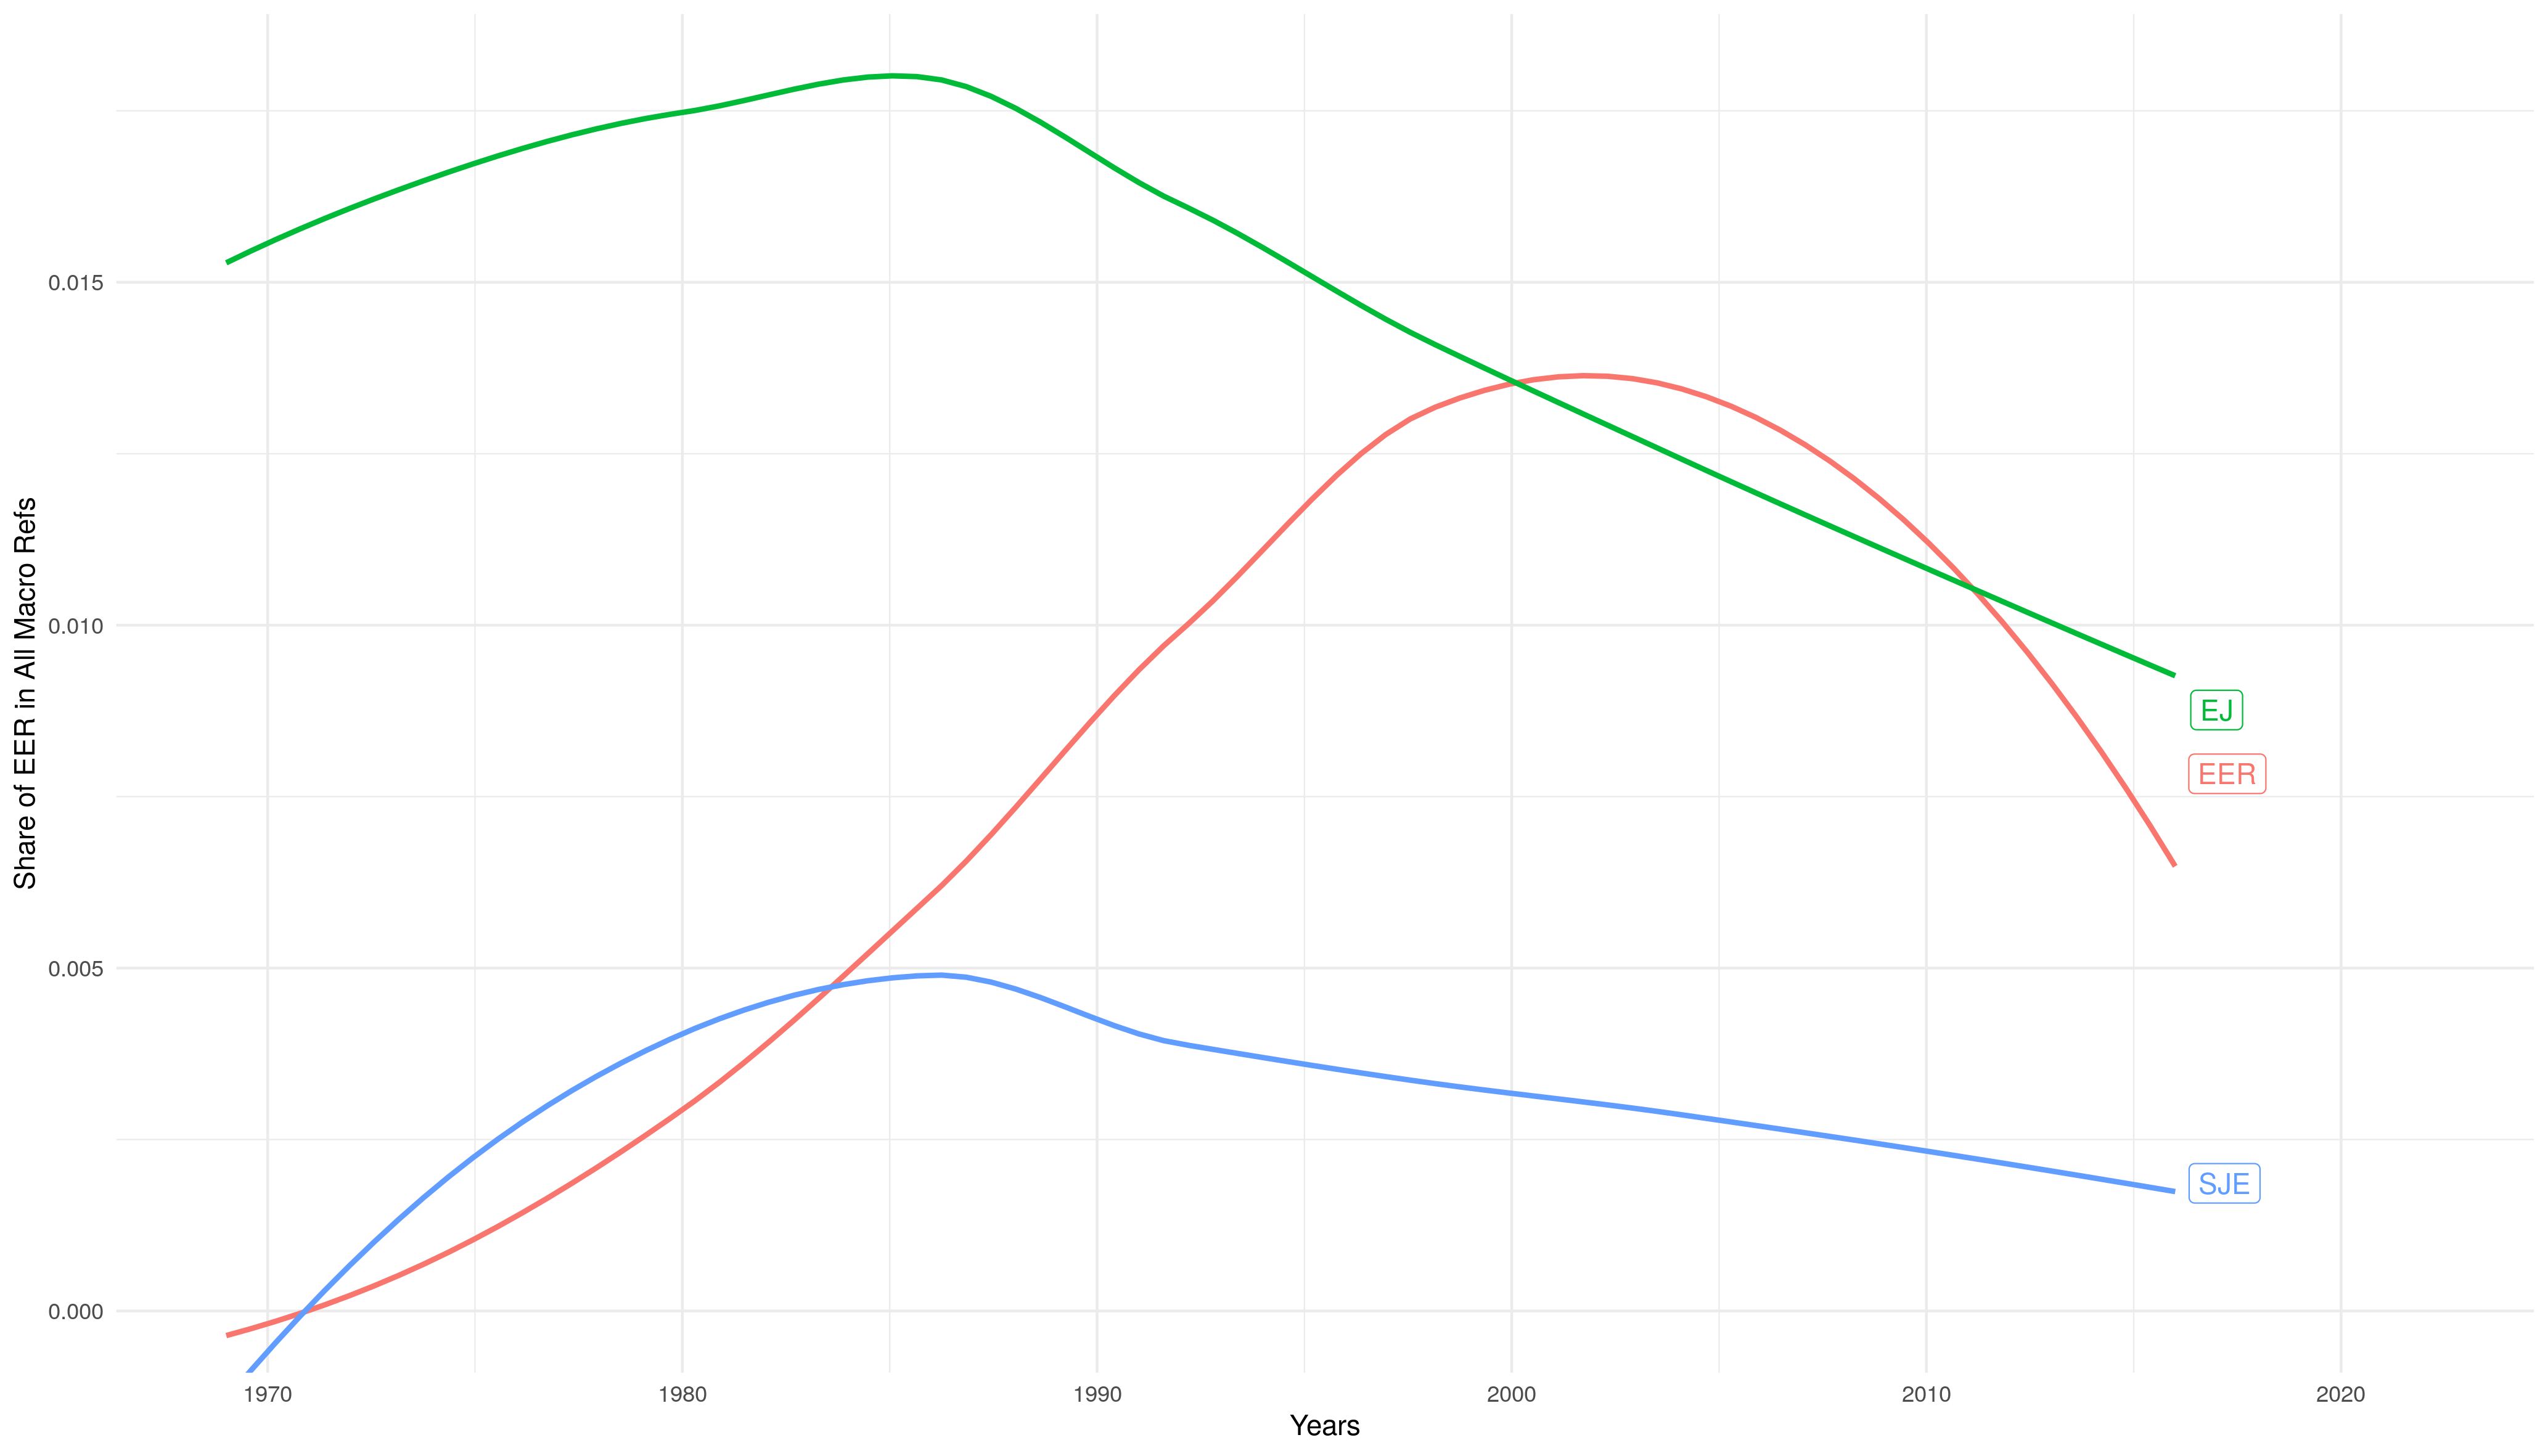
\includegraphics[width=1\linewidth]{G:/.shortcut-targets-by-id/1EHqA0pp2uozTykWv0_Stf5xyrvo_dkN5/data/EER/pictures/Graphs/EER_Importance} 

}

\caption{Share of total citations going to EER}\label{fig:plot-eer-importance}
\end{figure}

But has this whole process led to the total standardisation of a
European economics on the US model, or has it led to the development (or
persistence) of proper European specialities?

\hypertarget{european-specialities}{%
\section{Identifying European
Specialities}\label{european-specialities}}

\hypertarget{methods}{%
\subsection{Methods}\label{methods}}

The first step was to build our dataset. To identify European
specialities, we compare macroeconomics articles published in EER and in
the Top-5 journals, that is the \emph{American Economic Review}, the
\emph{Journal of Political Economy}, \emph{Econometrica}, the
\emph{Quarterly Journal of Economics} and the \emph{Review of Economic
Studies}. Focusing on the Top 5 allows us to only get the most popular
and dominant trends in macroeconomics and thus to draw clearer
comparisons with what is published in the EER. Besides, the EER was
created with the intent to establish an elite leading journal for the
European community that would imitate the standards of US major journal.
The Top 5 journals thus seem an adequate benchmark to compare the EER
to.

We identify macroeconomics articles by using the former and new JEL code
classification \citep{jel1991}.\footnote{See the complete list of all
  the JEL codes we have used in
  \protect\hyperlink{eer-top5-macro}{Appendix B.1.}.} Outside of JEL
codes data, we have used three different databases to collect different
types of information: outside of basic metadata (year of publication,
title, authors, \emph{etc.}), we have collected the list of
bibliographic references of EER and Top-5 articles, the abstracts, and
authors affiliations.\footnote{Crossing databases has been necessary due
  to missing years and information in the different databases we have
  used (Web of Science, Scopus and Microsoft Academic Premier). See the
  \protect\hyperlink{corpus}{Appendix B.1.} for more details on the
  building of our dataset.} Then, we have conducted two different types
of analysis to identify European specialities.

\hypertarget{bibliographic-coupling}{%
\subsubsection{Bibliographic coupling}\label{bibliographic-coupling}}

Bibliographic coupling connects articles together depending on the
bibliographic references they share. We build different networks of EER
and Top-5 articles (the nodes of the network), connected together by a
weighted edge, depending ib the number of references two articles share
together.\footnote{For more details on the measure of weights, see the
  \protect\hyperlink{network}{Appendix B.3.}.} We build networks on a
moving eight-year window (depending on the year of publication of the
articles). We thus have 23 networks from the 1973-1982 period, through
1974-1983, 1975-1984, \emph{etc.}, to the 1993-2002 period.{[}Due to
missing JEL codes for EER before 1973, we are forced to begin with the
1973-1982 window.{]} For each network, we use the Leiden algorithm
\citep{traag2019} to identify bibliographic clusters, that is groups of
articles that share many references in common, and few with articles
outside their cluster. Articles which belongs to the same cluster are
more likely to share cognitive content (e.g., sharing objects of study,
methods, results or theory) even if disagreeing
\citep{claveau2016, truc2021, goutsmedt2021}. Finally, we test the
similarity of the clusters two by two for successive time windows, and
merge clusters from different windows together when they are
sufficiently close.\footnote{See the
  \protect\hyperlink{network}{Appendix B.3.} for details on the merging
  criteria.}

This process allows us to obtain dynamic clusters Indeed, citation
patterns are highly dependent of the date of publication of an article:
scholars tend to cite more recent works. Consequently, for large time
window, clusters would likely be determined mainly by the publication
year, rather than by what they are talking about.\footnote{In other
  words, articles would be grouped together depending on the year of
  their publication and the clusterisation of the network would not say
  much of the economic content articles grouped together would share.}
By taking small time windows and then by merging communities in
different windows together, we avoid this problem and are able to
identify communities over longer period of time. We identify a total of
154 communities but only 33 are \emph{(i)} present in at least 2
networks (i.e.~two time windows) and \emph{(ii)} represent more than
0.04 percent of the nodes of at least one of the network they belong.

A set of indicators allows us to understand what these clusters are
about---e.g.~the words used in abstracts and titles, the recurrent
authors and the most cited references. These indicators help us to name
the clusters. For each cluster, we calculate the difference between the
mean of the cluster articles published in the EER and the same mean for
the Top 5. We do the same for the articles published by European-based
economists only, and those published by US-based economists only. These
two differences inform us on what are the most `Europeans' clusters,
meaning those where relatively more articles are published in the EER by
European-based economists.\footnote{Our assumption is that the content
  of articles published in the Top 5 by European economists could be
  more largely influenced by the standards of Top 5 journals and of US
  macroeconomics, and thus could be less representative of European
  economics than the articles published in the EER.} The figure
\ref{fig:plot-community-diff} display the position of each cluster
relatively to these two differences. When we sum the two differences, we
have a synthetic indicator of how much a cluster is European.

\begin{figure}[h]

{\centering \includegraphics[width=1\linewidth]{G:/.shortcut-targets-by-id/1EHqA0pp2uozTykWv0_Stf5xyrvo_dkN5/data/EER/pictures/Graphs/Communities_europeanisation_colored} 

}

\caption{The most European communities}\label{fig:plot-community-diff}
\end{figure}

\hypertarget{topic-modelling}{%
\subsubsection{Topic Modelling}\label{topic-modelling}}

Topic modelling is a non-supervised machine learning method which
associates \emph{(i)} the \emph{ngrams} contained in a corpus to
\emph{k} topics and \emph{(ii)} the documents of the corpus to the same
\emph{k} topics.\footnote{From the documents of our corpus, we extract
  (or `tokenise') unique words (or unigrams), bigrams and trigrams. Stop
  words are excluded and all words are `lemmatised'. See the
  \protect\hyperlink{topic}{Appendix B.4.} for more details on the
  preprocessing steps we use.} We have used a variant of the Latent
Dirichlet Allocation model with the Correlated Topic Model
\citep{blei2007}. The number of topics \emph{k} is chosen by the
modellers: after assessing quantitatively and qualitatively different
models, we choose to run the model with 50 topics.\footnote{The
  \protect\hyperlink{topic}{Appendix B.4.} gives more details on the
  different models we have tested and how we have set the number of
  topics.} For each topic, we can look at the word with the highest
`FREX' value \citep{bischof2012}.\footnote{FREX is the weighted harmonic
  mean of the terms' rank regarding exclusivity and frequency scores.
  Exclusivity is a measure of how much a term is frequent in a topic in
  comparison to its frequency in others. In other words, a good topic
  model is a model where the words in topics are frequently used, but
  each topic can be easily dinstinguished from others, for the words
  associated to this topic are scarce in other topics.} The Table
\ref{tab:summary-topics} displays the words with the highest FREX value
for each topic.

Similarly to what we do for bibliometric coupling, we are interested in
the topics characteristics regarding the publications (EER \emph{vs.}
Top 5) and the countries of affiliations of the authors (the US
\emph{vs.} European countries). As each article has a `rate of
belonging' to each topic (the \emph{gamma} value), we are able, for each
topic, to compute the difference in the means of \emph{gamma} values for
(i) articles published in the EER and articles published in the Top 5
and (ii) articles written by US-based authors and those written by
European-based authors. The resulting two differences are the
coordinates of the 50 topics in Figure \ref{fig:plot-topic-diff}. When
we sum the two differences, we have an indicator of how much a topic is
a European topic.

\begin{figure}[h]

{\centering \includegraphics[width=1\linewidth]{G:/.shortcut-targets-by-id/1EHqA0pp2uozTykWv0_Stf5xyrvo_dkN5/data/EER/pictures/topic_modelling/logratio_diff_plot} 

}

\caption{Topic Prevalence over journals (Difference of Means)}\label{fig:plot-topic-diff}
\end{figure}

\hypertarget{a-broad-picture-of-european-specialities}{%
\subsection{A Broad Picture of European
Specialities?}\label{a-broad-picture-of-european-specialities}}

In Section \ref{understanding-specialities}, we describe more in-depth
what we consider as three major European specialities. However, in a
first step, we can sketch a more general assessment of the peculiarities
of European macroeconomics.

First, topic modelling and bibliometric coupling allow us to understand
what European macroeconomics \emph{is not}. One of the first consistent
findings between the two methods is that the literature about the life
cycles and permanent income hypotheses, influenced by
\citet{friedman1957} and \citet{hall1978b}, was far from popular for
European economists. Close to this, the issue of debt, deficits and
agents' horizon stemming from Diamond's \citeyearpar{diamond1965},
Barro's \citeyearpar{barro1974}, and Blanchard's
\citeyearpar{blanchard1985} seminal papers, was also an unpopular issue
in Europe: topic 45 and the cluster ``Debts \& Deficits'' were among the
less European topics and clusters. Also, it took some time for Real
Business Cycles (RBC) to find the favours of European economists: the
first bibliographic cluster (going from the 1979-1988 window to the
1984-1993 window), ``RBC, fluctuations \& time series'' (see Table
\ref{tab:summary-communities}), was mostly a Top 5 / US-based community.
We find that the topic 14 on RBC was also clearly not
European.\footnote{The bibliometric analysis shows us that things have
  changed a bit after the mid-1990s, as a community on RBC (from
  1985-1994 to 1993-2002) was slightly European.}

We will focus on several results in the Section
\ref{understanding-specialities}. First, as exemplified by topics 21 and
51 (and perhaps also 24) as well as by the clusters ``Political Economy
of Central Banks'' and ``Monetary Policy \& Channels of Transmission'',
monetary policy and the role of central Banks represent a central issue
for European-based economists and for the EER (Section
\ref{central-banking}). Second, international macroeconomics seems more
represented in the European side (above all for topic-modelling). We
will focus on the topic 24 on the European Monetary system, which is
strongly linked with the clusters ``Exchange Rate Determination'' and
``Political Economy of Central Banks''.\footnote{For each topic, we can
  check to which clusters are belonging the articles with the highest
  \emph{gamma} value for this topic.} The question is to understand if
the concrete economic situation of European countries as pushed
European-based economists to investigate the issue differently than
their US colleagues (Section \ref{international-macro}). Finally, we
will investigate and clarfiy a strange paradox in our results. The
cluster on disequilibrium theory, imperfect competition and contracts is
by far the most European cluster, echoing Portes's
\citeyearpar{portes1987} assessment as well as
\citeyearpar{goutsmedt2021}. Nonetheless, there is no equivalent topic
and the same literature is split between several ones (topics 39, 53 and
47) which are not as ``European'' as the bibliographic cluster (Section
\ref{rigidities}).

Outside of the points cited above, it is worth noting the importance of
the issue of the explanation of unemployment, relying notably on
\citet{pissarides1990}, \citet{mortensen1994} and \citet{layard1991a}.
As for the most European topic (38), it seems not to form a really
consistent topic, but rather results from the aggregation of articles
using OECD data and comparing different countries notably by using
cross-country estimations. The conclusion we can draw from it is that
European-based economists and the EER appear more likely to welcome this
type of study.

\hypertarget{understanding-specialities}{%
\section{Understanding the European
Specialities}\label{understanding-specialities}}

\hypertarget{central-banking}{%
\subsection{A European Political Economy of Central
Banking?}\label{central-banking}}

\hypertarget{international-macro}{%
\subsection{A European International
Macroeconomics?}\label{international-macro}}

\hypertarget{rigidities}{%
\subsection{The many faces of microfoundations and
rigidities}\label{rigidities}}

\newpage

\hypertarget{references}{%
\section*{References}\label{references}}
\addcontentsline{toc}{section}{References}

\hypertarget{refs}{}
\begin{CSLReferences}{0}{0}
\end{CSLReferences}

\newpage

\hypertarget{appendices}{%
\section*{Appendices}\label{appendices}}
\addcontentsline{toc}{section}{Appendices}

\hypertarget{a---summary-tables}{%
\subsection*{A - Summary Tables}\label{a---summary-tables}}
\addcontentsline{toc}{subsection}{A - Summary Tables}

Here are the tables listing the different clusters and topics, with
their synthetic indicator of how much they are ``European''.

\begin{table}[!h]

\caption{\label{tab:summary-communities}Summary of Bibliographic Communities}
\centering
\fontsize{9}{11}\selectfont
\begin{tabular}[t]{lr}
\toprule
Communities & Differences\\
\midrule
\cellcolor{gray!6}{Modeling Consumption \& Production} & \cellcolor{gray!6}{2.0986873}\\
Disequilibrium \& Keynesian Macro & 2.0014930\\
\cellcolor{gray!6}{International Macroeconomics \& Target Zone} & \cellcolor{gray!6}{1.3359739}\\
Optimal Taxation 1 & 1.3235057\\
\cellcolor{gray!6}{Political Economics of Central Banks} & \cellcolor{gray!6}{1.0265264}\\
\addlinespace
Exchange Rate Dynamics & 0.7201769\\
\cellcolor{gray!6}{Taxation, Tobin's Q \& Monetarism} & \cellcolor{gray!6}{0.6388438}\\
Theory of Unemployment \& Job Dynamics & 0.5181369\\
\cellcolor{gray!6}{Capital \& Income Taxation} & \cellcolor{gray!6}{0.4078902}\\
Target Zone \& Currency Crises & 0.4058932\\
\addlinespace
\cellcolor{gray!6}{Coordination \& Sunspots 2} & \cellcolor{gray!6}{0.3465849}\\
Optimal Taxation 2 & 0.2787993\\
\cellcolor{gray!6}{Monetary Policy, Financial Transmission \& Cycles 2} & \cellcolor{gray!6}{0.2314883}\\
Business Cycles, Cointegration \& Trends & 0.2154401\\
\cellcolor{gray!6}{Taxation, Debt \& Growth} & \cellcolor{gray!6}{-0.0067936}\\
\addlinespace
Terms of Trade \& Devaluation & -0.0817679\\
\cellcolor{gray!6}{Endogenous Growth} & \cellcolor{gray!6}{-0.1105033}\\
RBC & -0.2094801\\
\cellcolor{gray!6}{Monetary Policy, Financial Transmission \& Cycles 1} & \cellcolor{gray!6}{-0.2379855}\\
Coordination \& Sunspots 1 & -0.3313256\\
\addlinespace
\cellcolor{gray!6}{Exchange Rate Dynamics \& Expectations} & \cellcolor{gray!6}{-0.4273431}\\
Monetary Policy, Target \& Output Gap & -0.6211658\\
\cellcolor{gray!6}{REH, Monetary Policy \& Business Cycles} & \cellcolor{gray!6}{-0.6758668}\\
Inflation, Interest Rates \& Expectations & -0.7403062\\
\cellcolor{gray!6}{Monetary Approach of Balance of Payments} & \cellcolor{gray!6}{-0.7658536}\\
\addlinespace
Credit Rationing, Rational Expectations \& Imperfect Information & -0.8270409\\
\cellcolor{gray!6}{Inflation \& Rigidities} & \cellcolor{gray!6}{-0.8396888}\\
Demand for Money & -0.8564033\\
\cellcolor{gray!6}{New Theory of Money: Search, Bargaining...} & \cellcolor{gray!6}{-1.2139877}\\
Permanent Income Hypothesis \& Life-Cycle & -1.4920219\\
\addlinespace
\cellcolor{gray!6}{Monetary Economics \& Demand for Money} & \cellcolor{gray!6}{-1.6768415}\\
Intergenerational Model, Savings and Consumption & -3.2194818\\
\cellcolor{gray!6}{Marginal Taxation} & \cellcolor{gray!6}{-3.3179236}\\
\bottomrule
\end{tabular}
\end{table}

\newpage

\begingroup\fontsize{9}{11}\selectfont

\begin{ThreePartTable}
\begin{TableNotes}
\item \textit{Note: } 
\item Differences values are the sum of (i) the difference in the gamma mean between EER and Top 5; (ii) the same difference but between European-based and US-based authors
\end{TableNotes}
\begin{longtable}[t]{>{}l>{}r>{\raggedright\arraybackslash}m{25em}}
\caption{\label{tab:summary-topics}Summary of Topics}\\
\toprule
Topics & Differences & Terms with the highest frex value\\
\midrule
\endfirsthead
\caption[]{Summary of Topics \textit{(continued)}}\\
\toprule
Topics & Differences & Terms with the highest frex value\\
\midrule
\endhead

\endfoot
\bottomrule
\insertTableNotes
\endlastfoot
Topic 46 & 0.030 & german;
money
demand;
germany;
unite
kingdom;
unite;
\cellcolor{gray!6}{kingdom}\\
Topic 22 & 0.026 & political;
oecd
country;
oecd;
world;
country;
index\\
Topic 6 & 0.024 & real
exchange;
real
exchange
rate;
exchange
rate;
flexible
exchange;
flexible
exchange
rate;
target
\cellcolor{gray!6}{zone}\\
Topic 25 & 0.023 & real
wage;
contract;
employment;
capacity;
wage;
stickiness\\
Topic 37 & 0.021 & unemployment;
job;
unemployment
rate;
creation;
flow;
phillips
\cellcolor{gray!6}{curve}\\
\addlinespace
Topic 3 & 0.014 & system;
monetary
expansion;
monetary
system;
union;
expansion;
stability\\
Topic 28 & 0.013 & exchange
market;
foreign
exchange
market;
intervention;
foreign
exchange;
transaction;
transaction
\cellcolor{gray!6}{cost}\\
Topic 39 & 0.013 & trade
balance;
trade;
wealth;
relative
price;
balance;
external\\
Topic 8 & 0.012 & credibility;
strategic;
policy;
maker;
economic
policy;
policy
\cellcolor{gray!6}{rule}\\
Topic 20 & 0.011 & inflation
target;
target;
stabilize;
central
bank;
central;
length\\
\addlinespace
Topic 45 & 0.009 & power
parity;
purchase
power
parity;
purchase
power;
power;
purchase;
\cellcolor{gray!6}{parity}\\
Topic 44 & 0.008 & level;
national
income;
inflationary;
equation;
price
level;
money
balance\\
Topic 40 & 0.006 & economic
growth;
growth
rate;
productivity
growth;
growth;
fast;
\cellcolor{gray!6}{region}\\
Topic 43 & 0.005 & federal;
signal;
monetary
policy;
federal
reserve;
revision;
feed\\
Topic 17 & 0.004 & indexation;
distortion;
labor
market;
labor;
product;
\cellcolor{gray!6}{corporate}\\
\addlinespace
Topic 11 & 0.003 & walrasian;
competitive;
temporary;
existence;
search;
equilibrium\\
Topic 30 & 0.003 & business
cycle;
business;
cycle;
real
business
cycle;
real
business;
\cellcolor{gray!6}{volatility}\\
Topic 31 & 0.002 & welfare
cost;
cost;
welfare;
bear;
survey;
household\\
Topic 13 & 0.001 & unanticipated;
activity;
economic
activity;
national;
economy;
\cellcolor{gray!6}{gap}\\
Topic 26 & 0.001 & inflation;
inflation
rate;
relative;
evidence;
dispersion;
nominal
price\\
\addlinespace
Topic 29 & 0.001 & capital
market;
mobility;
capital
mobility;
capital;
imperfect;
\cellcolor{gray!6}{intensity}\\
Topic 38 & 0.001 & asset
price;
financial
market;
stock
market;
return;
asset
market;
stock\\
Topic 4 & -0.001 & macroeconomics;
rich;
history;
robert;
divide;
\cellcolor{gray!6}{lead}\\
Topic 34 & -0.001 & plan;
stage;
multiple
equilibrium;
option;
crisis;
currency\\
Topic 15 & -0.002 & production;
class;
factor;
identical;
preference;
\cellcolor{gray!6}{input}\\
\addlinespace
Topic 23 & -0.002 & short
run;
run;
short;
burden;
indirect;
externality\\
Topic 24 & -0.002 & term;
spread;
short
term;
term
structure;
premium;
\cellcolor{gray!6}{structure}\\
Topic 36 & -0.002 & spend;
government
spend;
deficit;
fiscal;
government;
government
debt\\
Topic 47 & -0.002 & investment;
monopolistic;
dynamic;
competition;
macroeconomic;
\cellcolor{gray!6}{replace}\\
Topic 50 & -0.002 & budget
constraint;
constraint;
project;
budget;
bad;
loan\\
\addlinespace
Topic 35 & -0.004 & likelihood;
variable;
estimation;
autoregressive;
variance;
endogenous
\cellcolor{gray!6}{variable}\\
Topic 18 & -0.005 & generation;
overlap;
overlap
generation;
social
security;
live;
generation
model\\
Topic 48 & -0.005 & liquidity;
credit;
debt;
insurance;
access;
\cellcolor{gray!6}{investor}\\
Topic 32 & -0.006 & standard;
gold;
dollar;
reserve;
price
level;
size\\
Topic 1 & -0.007 & inventory;
hold;
association;
century;
create;
\cellcolor{gray!6}{rationally}\\
\addlinespace
Topic 5 & -0.007 & price
adjustment;
oil;
price;
commodity
price;
sticky;
import\\
Topic 21 & -0.007 & process;
procedure;
property;
incentive;
build;
\cellcolor{gray!6}{endogenous}\\
Topic 9 & -0.008 & skill;
asymmetric
information;
program;
change;
research;
complementarity\\
Topic 27 & -0.008 & perfect
foresight;
foresight;
time
vary;
time;
perfect;
continuous
\cellcolor{gray!6}{time}\\
Topic 41 & -0.008 & optimal;
optimal
tax;
growth
model;
function;
optimal
policy;
optimal
\cellcolor{gray!6}{taxation}\\
\addlinespace
Topic 49 & -0.008 & report;
composition;
regime;
critique;
puzzle;
\cellcolor{gray!6}{profit}\\
Topic 7 & -0.010 & control;
stochastic;
game;
equivalence;
equivalent;
solution\\
Topic 42 & -0.010 & stationary;
rational
expectation
equilibrium;
expectation
equilibrium;
expectation;
unique;
rational
\cellcolor{gray!6}{expectation}\\
Topic 33 & -0.012 & depression;
theory;
subsequent;
classical;
pure;
principle\\
Topic 12 & -0.015 & lm;
risk
aversion;
utility
function;
aversion;
intertemporal;
\cellcolor{gray!6}{risk}\\
\addlinespace
Topic 2 & -0.017 & money
supply;
money
stock;
money;
fix
exchange;
supply;
fix
exchange
rate\\
Topic 10 & -0.018 & tax;
capital
income;
income
tax;
tax
system;
redistribution;
income
taxation\\
Topic 16 & -0.018 & public;
strategy;
finance;
local;
provision;
desirable\\
Topic 19 & -0.021 & expect
rate;
cash;
sargent;
nominal;
expect
inflation;
\cellcolor{gray!6}{expect}\\
Topic 14 & -0.022 & income
distribution;
labor
income;
permanent;
sensitivity;
permanent
income;
income\\*
\end{longtable}
\end{ThreePartTable}
\endgroup{}

\newpage

\hypertarget{appendix}{%
\subsection*{B - Information on the Methods}\label{appendix}}
\addcontentsline{toc}{subsection}{B - Information on the Methods}

\hypertarget{corpus}{%
\subsubsection*{B.1. Corpus Creation}\label{corpus}}
\addcontentsline{toc}{subsubsection}{B.1. Corpus Creation}

For the present study we used two different corpora. The first corpus is
composed of all EER articles and allows us to track how publications,
citations, references and authors affiliations evolved since the
creation of the journal in 1969 up to the 2002. The second corpus is
composed of all macroeconomic articles published in the top five
economics journals and the EER. Macroeconomic articles are identified
thanks to the former and new classification of the JEL codes
\citep{jel1991}.\footnote{See \ref{eer-top5-macro} for the list of JEL
  codes used.} This is used as the basis for topic modeling and
bibliographic coupling analysis to contrast the top macroeconomics
publications authored by European-based and US-based authors, and/or
published in top 5 journals and in the EER.

\hypertarget{eer-publications}{%
\paragraph*{EER Publications}\label{eer-publications}}
\addcontentsline{toc}{paragraph}{EER Publications}

For the creation of the first corpus composed of all EER articles, we
used a mix of \emph{Web of Science} (WoS) and \emph{Scopus}. While WoS
has all articles of the EER between 1969-1970 and 1974-2002, it is
missing most articles published between 1971 and 1973. To make up for
the missing data, we use Scopus to complete the dataset. This operation
required normalization of the Scopus dataset, and manual cleaning of
variables that were missing from Scopus compared to WoS. This mostly
includes cleaning the references to match \emph{Scopus} references with
WoS ones, and identification of author's affiliation.

Moreover, given that the size of our corpus is modest, we made an
extensive semi-automatic cleaning of references to improve references
identification by adding the most commonly cited books, book chapter,
and articles that are not otherwise identified in WoS when possible.

\hypertarget{eer-top5-macro}{%
\paragraph*{EER and Top 5 Macroeconomics
Articles}\label{eer-top5-macro}}
\addcontentsline{toc}{paragraph}{EER and Top 5 Macroeconomics Articles}

The construction of this corpus is made in multiple steps:

\begin{enumerate}
\def\labelenumi{\arabic{enumi}.}
\item
  Identifying macroeconomics articles

  \begin{itemize}
  \item
    We identified all articles published in macroeconomics using JEL
    codes related to macroeconomics (we get JEL codes of Top 5 and EER
    articles thanks to the Econlit database). We consider that an
    article is a macroeconomics article if it has one of the following
    codes:

    \begin{itemize}
    \tightlist
    \item
      For old JEL codes (pre-1991): 023, 131, 132, 133, 134, 223, 311,
      313, 321, 431, 813, 824.
    \item
      For new JEL codes (1991 onward): all E, F3 and F4.\footnote{The
        new classification has a clear categorisation of Macroeconomics
        (the letter `E'), but we had F3 and F4 as they deal with
        international macroeconomics. For the older JEL codes, we use
        the table of correspondence produce by the \emph{Journal of
        Economic Literature} itself \citep{jel1991}.}.
    \end{itemize}
  \end{itemize}
\item
  Using these JEL codes, we match econlit articles with WoS articles
  when they shared the same:

  \begin{itemize}
  \tightlist
  \item
    Journal, Volume, First Page
  \item
    Year, Journal, First Page, Last Page
  \item
    Year, Volume, First Page, Last Page
  \item
    First Author, Year, Volume, First Page
  \item
    First Author, Title, Year
  \item
    Title, Year, First Page
  \end{itemize}
\end{enumerate}

Out of the 3592 articles we get in econlit, we matched 3428 of them in
WoS.\footnote{Most of the unmatched articles are not `articles' properly
  speaking: they often are reply and comments on other published
  articles. (Investigate this deeper)}

\begin{enumerate}
\def\labelenumi{\arabic{enumi}.}
\setcounter{enumi}{2}
\item
  Using this list of articles in WoS, we took all articles in
  macroeconomics published in the EER (Corpus 1 improved with Scopus)
  and in the top five journals (\emph{American Economic Review},
  Econometrica, \emph{Review of Economic Studies}, \emph{Journal of
  Political Economy}, \emph{Quarterly Journal of Economics}).
\item
  Finally, we were able to collect abstracts:

  \begin{itemize}
  \tightlist
  \item
    using \emph{Scopus} for the EER. All abstracts have been matched
    with the EER corpus.
  \item
    using \emph{Microsoft Academics} to collect the highest number of
    available abstracts for the Top 5 as too many abstracts were missing
    in WoS or \emph{Scopus}. The abstracts extracted from this database
    are matched with our WoS Top 5 corpus using
  \end{itemize}
\end{enumerate}

\hypertarget{b.2.-variable-creation}{%
\subsubsection*{B.2. Variable creation}\label{b.2.-variable-creation}}
\addcontentsline{toc}{subsubsection}{B.2. Variable creation}

\hypertarget{author-affiliation}{%
\paragraph*{Authors' affiliation}\label{author-affiliation}}
\addcontentsline{toc}{paragraph}{Authors' affiliation}

Authors' affiliations information were extracted from WoS. However, the
affiliations are not per author, but instead per institutional
departments per paper. For example, in the case of an article with two
authors from the same department, the department (and institution or
country associated with it) is only counted once. Similarly, a
single-authored article where the author has three affiliations can
result in one article having three affiliations. While in some cases we
can inferred the institutional affiliation for each author (e.g., one
institution, multiple authors), in others we cannot (e.g., two
institutions, three authors). For example, in an article with two
authors from Princeton and one author from Stanford, we only know that
the article was written by at least one author from Princeton and at
least one from Stanford, but not that the individual ratio was two
third.

We restructure the information in two ways.

First, for each article, we only kept one occurrence of each unique
institutions (university, research institutes\ldots) to avoid the
multiplication of observations resulting from the variety of departments
observed in some institutions. In other words, for each article, authors
are group by their institutional affiliation not by their department or
research team.

Second, and more importantly, for the purpose of our analysis, we mostly
looked at the share of papers authored by European-based and US-based
economists. While we do not have individual affiliation, we know with
certainty when a paper has only European authors, only American authors,
or a mix of the two. For this reason, while the share of institutions
within the corpus is only an estimation based on the occurrences of
affiliation, the information generated to identify US authored papers
and European authored paper is certain.

\hypertarget{network}{%
\subsubsection*{B.3. Bibliographic Coupling and Cluster
Detection}\label{network}}
\addcontentsline{toc}{subsubsection}{B.3. Bibliographic Coupling and
Cluster Detection}

A first way to identify potential differences between European and
American macroeconomics is to find articles written by Europeans and
published in European journals, resembling each others but dissimilar to
American articles. To do that, we used bibliographic coupling
techniques. In a bibliographic coupling network, a link is created
between two articles when they have one or more references in common.
The more references that two articles have in common, the stronger the
link. Bibliographic coupling is one way to measure how similar two
articles are in a corpus. To normalize and weight the link between two
articles, we used the refined bibliographic coupling strength of
\citet{shen2019}. This method normalized and weight the strength between
articles by taking into account two important elements

\begin{enumerate}
\def\labelenumi{\arabic{enumi}.}
\tightlist
\item
  The size of the bibliography of the two linked articles. It means that
  common references between two articles with long bibliography are
  weighted as less significant since the likeliness of potential common
  references is higher. Conversely, common references between two
  articles with a short bibliography is weighted as more significant.
\item
  The number of occurrences of each reference in the overall corpus.
  When a reference is shared between two articles, it is weighted as
  less significant if it is very common reference across the entire
  corpus and very significant if it is scarcely cited. The assumption is
  that a very rare common reference points to a higher content
  similarity between two articles than a highly cited reference.
\end{enumerate}

For all macroeconomics articles published in the EER and in the Top 5,
we build the networks with \texttt{time\_window}-year overlapping
windows. This results in 23.

We used Leiden detection algorithm \citep{traag2019} that optimize the
modularity on each network to identify groups of articles that are
similar to each others and dissimilar to the rest of the network. We use
a resolution of 1 with 1000 iterations. This results in 466 across all
networks. Because networks have a lot of overlaps, many clusters between
two periods are composed of the same articles. To identify these
clusters that are very similar between two time windows, we considered
that \emph{(i)} if at least 55\% of the articles in a community of the
first time window where in the same cluster in the second time window,
and that \emph{(ii)} if the cluster was also composed by at least 55\%
of articles of the first time window, \emph{then} it is the same cluster

Simply put, if two clusters share a high number of articles, and are
both mostly composed by these shared articles, they are considered the
same cluster.

This gives us 154, with 33 that are at least 0.04\% of a network at any
given point and are stable enough to exists for at least 2 time windows.

For each clusters, we identified the American or European oriented
nature of its publications and authors. A first measure we used is the
over/under representation of European/American authors in the cluster.
For each cluster, we subtracted the relative share of European authors
to American authors in the cluster, to the relative share of European
authors to American on the same time window of the cluster leading us to
the first index:\newline

\(\text{Author EU/US Orientation}=\log(\frac{\text{Share Of European Authored Articles In The Cluster}}{\text{Share Of American Authored Articles In The Cluster}})-\log(\frac{\text{Share Of European Authored Articles In The Time Window}}{\text{Share Of American Authored Articles In The Time Window}})\)\newline

We then use a second similar index for the publication venue of the
articles in the cluster. For each cluster, we subtracted the relative
share of EER publications to Top 5 publications in the cluster, to the
relative share of EER publications to Top 5 publications on the same
time window of the cluster:\newline

\(\text{Journal EU/US Orientation}=\log(\frac{\text{Share Of EER Articles In The Cluster}}{(1-\text{Share Of EER Articles In The Cluster})})-\log(\frac{\text{Share Of EER Articles In The Time Window}}{(1-\text{Share Of EER Articles In The Time Window})})\)\newline

To get an overall index score of the European/US orientation of
clusters, we simply sum the two previous index:\newline

\(\text{Overall EU/US Orientation}=\text{Author EU/US Orientation} + \text{Journal EU/US Orientation}\)\newline

Finally, clusters are placed on a scatterplot with the Y-axis for the
EER vs Top 5 score, and the X-Axis for the American vs European authors
score. The size of the points captures the size of the cluster with the
number of articles that are in it, and the color of the cluster is
simply the sum of the two Y and X scores.

\hypertarget{topic}{%
\subsubsection*{B.4. Topic Modelling}\label{topic}}
\addcontentsline{toc}{subsubsection}{B.4. Topic Modelling}

\hypertarget{preprocessing}{%
\paragraph*{Preprocessing}\label{preprocessing}}
\addcontentsline{toc}{paragraph}{Preprocessing}

We have several steps to clean our texts before running our topic
models:

\begin{enumerate}
\def\labelenumi{\arabic{enumi}.}
\tightlist
\item
  Once we have our corpus, we merge titles and abstracts together for
  all EER and Top 5 articles.
\item
  We use the \emph{tidytext} and \emph{tokenizers} R packages to
  `tokenise' the resulting texts (when there is no abstract, only the
  title if thus tokenise)?\footnote{See Silge J, Robinson D (2016).
    ``tidytext: Text Mining and Analysis Using Tidy Data Principles in
    R.'' \emph{JOSS}, \emph{1}(3) and Lincoln A. Mullen et al., ``Fast,
    Consistent Tokenization of Natural Language Text,'' Journal of Open
    Source Software 3, no.23 (2018): 655.} Tokenisation is the process
  of transforming human-readable text into machine readable objects.
  Here, the text is split in unique words (unigrams), bigrams (pair of
  words) and trigrams. In other words, to each article is now associated
  a list of unigrams, bigrams and trigrams, some appearing several times
  in the same title + abstract.
\item
  Stop words are removed using the \emph{Snowball}
  dictionary.\footnote{See
    http://snowball.tartarus.org/algorithms/english/stop.txt.} We add to
  this dictionary some current verbs in abstract like ``demonstrate'',
  ``show'', ``explain''. Such verbs are likely to be randomly
  distributed in abstracts, but we want to limit the noise as much as
  possible.
\item
  We lemmatise the words using the \emph{textstem} package.\footnote{Rinker,
    T. W. (2018). textstem: Tools for stemming and lemmatizing text
    version 0.1.4. Buffalo, New York.} The lemmatisation is the process
  of grouping words together according to their ``lemma'' which depends
  on the context. For instance, different form of a verb are reduced to
  its infinitive form. The plural of nouns are reduced to the singular.
\end{enumerate}

\hypertarget{choosing-the-number-of-topics}{%
\paragraph*{Choosing the number of
topics}\label{choosing-the-number-of-topics}}
\addcontentsline{toc}{paragraph}{Choosing the number of topics}

We use the Correlated Topic Model \citep{blei2007} method implemented in
the \emph{STM} R package.\footnote{Roberts ME, Stewart BM, Tingley D
  (2019). ``stm: An R Package for Structural Topic Models.''
  \emph{Journal of Statistical Software}, \emph{91}(2), 1-40.}

From the list of words we have tokenised, cleaned and lemmatised, we
test different thresholds and choices by running different models:

\begin{itemize}
\tightlist
\item
  by exluding trigrams or not;
\item
  by removing the terms that are present in less than 0.5\% of the
  Corpus (17), 1\% (34) and 2\% (68);
\item
  by removing articles with less than 6 words or with less than 12
  words.\footnote{Here, only articles with no abstract are impacted.}
\end{itemize}

Crossing all these criteria, we thus have 12 different possible
combinations. For each of these 12 different combinations, we have run
topic models for different number of topics from 20 to 110 with a gap of
5. The chosen model integrates trigram, removes only terms that appear
in less than 0,5\% of the documents and keep all articles if they have
more than 6 words in their title + abstract. We choose to keep the model
with 55 topics.

We have chosen the criteria and the number of topics by comparing the
performance of the different models in terms of the FREX value
\citep{bischof2012}.

\bibliography{bibliography.bib}


\end{document}
